\documentclass[11pt]{article}
\usepackage[utf8]{inputenc}
\usepackage[ngerman]{babel}

\usepackage{amsmath,amsthm,amssymb,amsfonts}

\usepackage{graphicx}
\usepackage{float}
\usepackage{tikz}

\usepackage{fancyhdr} % For headers and footers
\usepackage{geometry}
\usepackage{listings}
\usepackage{hyperref}
\hypersetup{
    linkcolor=blue,     
    urlcolor=cyan,
}

\geometry{
    a4paper, % Change this if you intend to print on a different paper size, such as letter paper.
    left=20mm,
    right=20mm,
    top=30mm,
    bottom=30mm,
}

\newcount\colveccount
\newcommand*\colvec[1]{
        \global\colveccount#1
        \begin{pmatrix}
        \colvecnext
}
\def\colvecnext#1{
        #1
        \global\advance\colveccount-1
        \ifnum\colveccount>0
                \\
                \expandafter\colvecnext
        \else
                \end{pmatrix}
        \fi
}

\title{Dynamik - Drehmoment (Rotation)}
\author{Emil Staikov}
\date{31. Mai 2021}

\begin{document}
\maketitle
Der erste Schritt in der Untersuchung der Dynamik der Rotationsbewegung ist sich zu überlegen, was passiert, wenn eine Kraft auf einen Körper wirkt, der an einer festen Drehachse hängt. Dafür erschließen wir uns zuerst das Konzept eines Hebels. 

\section{Hebel}
\begin{figure}[H]
        \centering
        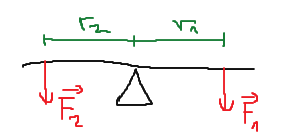
\includegraphics[]{abb/6-rotation-drehmoment/wippe.png}
        \caption{Wippe als Beispiel für einen Hebel.}
\end{figure}

Experimentell finden wir, dass die Wippe im Gleichgewicht ist, wenn $r_1F_1 = r_2F_2$ gilt, wobei wir hier nur die Kraftkomponente betrachten, die senkrecht zum Radius steht. Die Wippe können wir als Rotationsbewegung um den Auflagepunkt verstehen, die Größe $rF\sin(\varphi)$ definieren wir als Drehmoment $M$ mit $[M] = Nm$, wobei $\varphi$ der Winkel zwischen $r$ und $F$ ist. 

\section{Drehmoment bei Rotationsbewegungen}
Wenn eine Kraft auf ein mit einer Drehachse verbundenes Objekt wirkt, so ist der Effekt dieses Anstoßens von dem Abstand des Objekts von der Drehachse abhängig. Daher ist es sinnvoll bei Drehbewegungen mit dem Drehmoment zu rechnen, damit beziehen wir den Faktor Radius mit ein. In der Rotationsbewegung ist das Drehmoment analog zur Kraft in der Translationsbewegung. \\\\
Die Kraftkomponente, die zu einer Bewegung führt, steht senkrecht zum Radius. Wenn eine Kraft entlang des Radius wirkt, so führt das bei fixierter Drehachse zu keiner Bewegung. Das kann man auch ausprobieren, eine Tür bewegt sich, wenn man sie senkrecht zu ihrer Oberfläche anschiebt. Wenn man jedoch in Richtung der Scharniere Kraft ausübt, wird sie sich nicht bewegen. 
\begin{figure}[H]
        \centering
        \includegraphics{abb/6-rotation-drehmoment/kraftrichtung-tür.png}
        \caption{$F_1$ hat keine Änderung der Rotationsbewegung zur Folge, $F_2$ hingegen schon.}
\end{figure}

\section{Das 2. Newton'sche Axiom der Rotationsbewegung}
Betrachten wir einen Massepunkt (Körper mit vernachlässigbarer Größe) mit Masse $m$ im festen Abstand $r$ von einer fixierten Drehachse. Wir üben eine Kraft $F$ senkrecht zum Radius aus. Dann wirkt folgendes Drehmoment auf den Massepunkt
\begin{align*}
        M = rF = rma = rmr\alpha = mr^2\alpha
\end{align*}
Hier ist $\alpha$ die Winkelbeschleunigung. \\\\
Das der Kraft entsprechende Drehmoment hängt also mit der der Beschleunigung entsprechenden Winkelbeschleunigung durch den Faktor $mr^2$ zusammen. Diese Größe definieren wir als das Trägheitsmoment $I$ des Massepunkts, $[I] = kgm^2$. Wenn wir uns an das 2. Newton'sche Axiom, $F = ma$, zurückerinnern, so scheint das Trägheitsmoment bei der Rotationsbewegung der Masse bei der Translationsbewegung zu entsprechen. \\
Das ist auch anschaulich sinnvoll, die Masse kann man als Maß der Trägheit gegenüber der Beschleunigung verstehen. Wenn wir versuchen einen Körper zu drehen, wird dies schwerer, je mehr Masse weiter von der Drehachse entfernt ist. Das Trägheitsmoment ist für größere Masse mit größerem Abstand von der Drehachse ebenfalls größer. \\\\
Das Trägheitsmoment $I$ können wir auch auf $n$ Massepunkte mit Masse $m_i$ im Abstand $r_i$ verallgemeinern:
\begin{equation*}
        I = \sum_{i=1}^n m_ir_i^2
\end{equation*}
Äquivalent zu der Herleitung für einen Massepunkt ergibt sich der Zusammenhang zwischen Drehmoment, Winkelbeschleunigung und Trägheitsmoment: 
\begin{equation*}
        M = I\alpha
\end{equation*}
Dies entspricht inhaltlich dem schon bekannten 2. Newton'schen Axiom 
\begin{equation*}
        F = ma
\end{equation*}
und wird daher auch als das 2. Newton'sche Axiom der Rotationsbewegung bezeichnet. 

\end{document}
